\documentclass[border=10pt]{standalone}

\usepackage{tikz}
\usepackage{tikzsymbols}
\usetikzlibrary{calc,patterns,shapes.geometric}

\def\centerarc[#1](#2)(#3:#4:#5){\draw[#1] ($(#2)+({#5*cos(#3)},{#5*sin(#3)})$) arc (#3:#4:#5);}

\begin{document}
	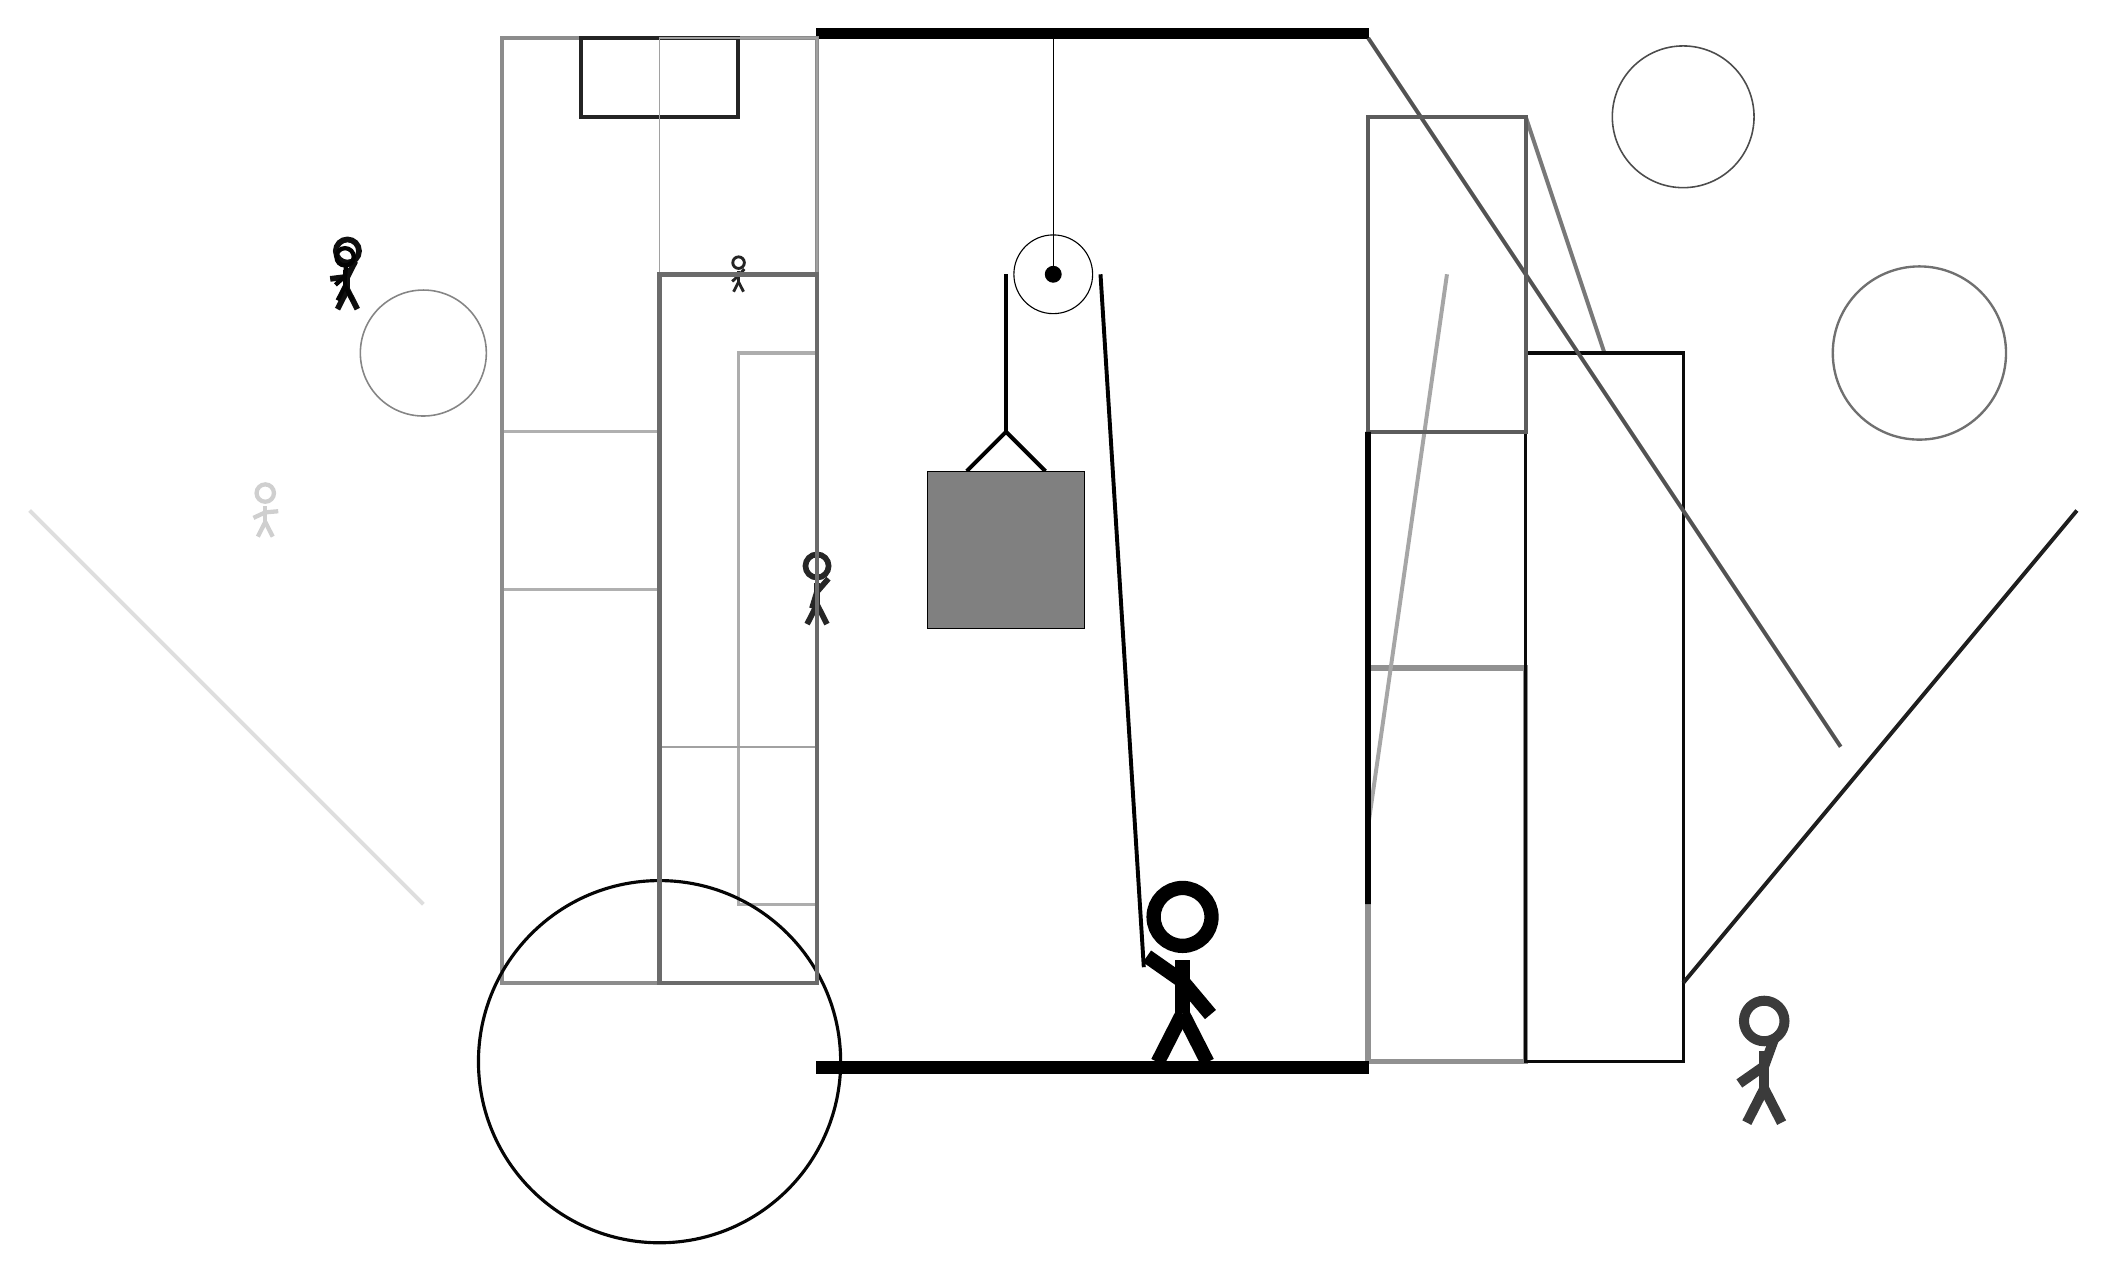
\begin{tikzpicture}
		%%%%% START %%%%%
		
		\draw[fill=black] (-2, 10) rectangle (5, 10.125);
		
		\draw (1, 7) circle (0.5);
		\draw[fill=black] (1, 7) circle (0.1);
		\draw (1, 10) -- (1, 7);
		
		\draw[line width=0.5mm] (-0.1, 4.5) -- (0.4, 5.0) -- (0.9, 4.5);
		\draw[fill=black!50] (-0.6, 4.5) rectangle (1.4, 2.5);
		
		\draw[line width=0.7mm, color=black!36] (-4, 3) rectangle (-4, 4);
		
		\node[line width=0.4mm, color=black!77] at (10, -3) {\Strichmaxerl[7][35][70]};
		\node[line width=0.3mm, color=black!19] at (-9, 4) {\Strichmaxerl[3][25][5]};
		\node[line width=0.5mm, color=black!94] at (-8, 7) {\Strichmaxerl[4][7][63]};
		
		\draw[line width=0.5mm, color=black!13](-7, -1) -- (-12, 4);
		\draw[line width=0.4mm, color=black!31] (-4, 5) rectangle (-6, 3);
		
		\draw[line width=0.6mm, color=black!45] (-2, 10) rectangle (-6, -2);
		
		\node[line width=0.4mm, color=black!99] at (-8, 7) {\Strichmaxerl[3][42][85]};
		\draw[line width=0.7mm, color=black!43] (5, 2) rectangle (7, -3);
		\draw[line width=0.5mm, color=black!53](8, 6) -- (7, 9);
		\draw [line width=0.2mm, color=black!70](9, 9) circle (0.9);
		
		\draw[line width=0.4mm, color=black!32] (-3, -1) rectangle (-2, 6);
		\draw[line width=0.4mm, color=black!96] (7, -3) rectangle (9, 6);
		
		\node[line width=0.6mm, color=black!85] at (-2, 3) {\Strichmaxerl[4][73][49]};
		\draw [line width=0.4mm, color=black!98](-4, -3) circle (2.3);
		\draw[line width=0.5mm, color=black!35](5, 0) -- (6, 7);
		
		\draw[line width=0.5mm, color=black!68](5, 10) -- (11, 1);
		\draw[line width=0.5mm, color=black!86] (-3, 10) rectangle (-5, 9);
		\draw [line width=0.3mm, color=black!56](12, 6) circle (1.1);
		
		\node[line width=0.4mm, color=black!86] at (-3, 7) {\Strichmaxerl[2][43][48]};
		\draw[line width=0.5mm, color=black!88](9, -2) -- (14, 4);
		\draw[line width=0.2mm, color=black!37] (-2, 10) rectangle (-4, 1);
		\draw[line width=0.5mm, color=black!64] (5, 9) rectangle (7, 5);
		\draw [line width=0.2mm, color=black!73](13, 1) circle (0.0);
		\draw[line width=0.7mm, color=black!99] (5, 5) rectangle (5, -1);
		
		\draw [line width=0.2mm, color=black!48](-7, 6) circle (0.8);
		\draw[line width=0.6mm, color=black!58] (-2, -2) rectangle (-4, 7);
		
		\draw[line width=0.5mm] (0.4, 7) -- (0.4, 5.0);
		\centerarc[line width=0.5mm](1, 7)(0:180:0.6);
		\draw[line width=0.5mm](1.6, 7) -- (2.15, -1.8);
		
		\node at (2.6, -1.9) {\Strichmaxerl[10][-35][-50]};
		
		\draw[fill=black] (-2, -3) rectangle (5, -3.15);
		
		%%%%% END %%%%%
	\end{tikzpicture}
\end{document}